
\section{Class Introduction}
\subsection{Outline}

\begin{frame}
  \centering
  {\huge
    Course Introduction
  }
\end{frame}

% \begin{frame}
%   \frametitle{Outline}
%   \begin{enumerate}
%     \item Course Objective
%     \item What is a Programming Challenge?
%     \item Course Topics
%     \item Lecturer Introduction
%     \item Extra: ICPC
%   \end{enumerate}
% \end{frame}

\subsection{Class Objective}
\begin{frame}{What is the goal of this course?}
  \begin{itemize}
    \item \alert{Course Objective}: Improve your skill by writing many programs;
    \bigskip

    \item \alert{How?} Write a program that solves a puzzle (programming challenge)
      \medskip
    \begin{enumerate}
      \item Read and understand the puzzle;
      \item Think what program solves the puzzle;
      \item Write the program;
      \item Test the result of the program;
    \end{enumerate}
    \medskip

    \item \alert{Why?} 
    \begin{enumerate}
      \item We use in practice the algorithms learned in the second year.
      \item We learn how the algorithm works in practice.
      \item We learn how to debug from data.
    \end{enumerate}

  \end{itemize}
\end{frame}

% \begin{frame}{Learning Algorithms: Theory vs. Implementation}
%   \begin{exampleblock}{}
%     When we implement an algorithm in a hard program we learn many things:
%   \end{exampleblock}
%   \begin{itemize}
%     \item \alert{Input/Output}: How to prepare the input data for the algorithm to use it;
%     \item \alert{Input Size}: Relationship between input size, algorithm, and program speed;
%     \item \alert{Special Cases}: Difficult Input Data that causes bugs;
%     \item \alert{Debugging}: How to find bugs by yourself;
%   \end{itemize}
% \end{frame}

\begin{frame}{Automated Judge (AJ)}
  \begin{exampleblock}{}
    This course uses an \alert{Automated Judge (AJ)} to check your homework.
  \end{exampleblock}

  \begin{itemize}
  \item An AJ is a program that checks if code is correct:
    \begin{itemize}
      \item Ex: AtCoder, Aizu Online Judge, Topcoder, Codeforces, etc.
    \end{itemize}\bigskip

  \item The AJ checks your program agains \alert{Secret Test Data}.\bigskip

  \item The AJ tells you if your code is \alert{correct or incorrect}.
  \end{itemize}

  \begin{alertblock}{When your program is incorrect: Be Careful!}
    \begin{itemize}
      \item Debug your program carefully;
      \item Create your own test data;
      \item Think before submitting again;
    \end{itemize}
  \end{alertblock}
\end{frame}

\begin{frame}{Class Requirements}
  \begin{exampleblock}{}
    \begin{itemize}
    \item You have basic programming knowledge (C++, Java or Python);
      \begin{itemize}
      \item This is a hard \alert{programming} class
      \item Data structures and algorithms are important
      \end{itemize}
      \medskip

    \item You will do homework every week;
      \begin{itemize}
        \item Minimum 2 programs per week; 
        \item Debug carefully;
      \end{itemize}
      \medskip

      \item You will not copy the homework;
      \begin{itemize}
        \item Copy homework from other students will be penalized;
        \item Copy homework from the internet will be penalized;
        \item Penalties include failing the course, and failing the semester;
      \end{itemize}
      \medskip

      \item No final exam -- only homework
    \end{itemize}
  \end{exampleblock}
  \hfill {Hint: Do your homework early!}
\end{frame}

\subsection{What are Programming Challenges?}
\begin{frame}{Homework: What are Programming Challenges?}

  It is a puzzle that you solve by writing a program.
  \bigskip

  The program reads the input, and must write the correct output.
  \begin{itemize}
  \item Difficulty 1: The output must be \alert{exactly} correct.
  \item Difficulty 2: The test input is \alert{not known}.
  \item Difficulty 3: There is a maximum \alert{execution time}.
  \end{itemize}\bigskip

  In general, a correct program will be small (< 200 lines).
\end{frame}

\subsection{Example}
\begin{frame}{Programming Challenge Example: "The 3n+1 problem"}
  \begin{columns}
    \column{0.55\textwidth}
      Contents of a Programming Challenge:
      \begin{itemize}
        \item Problem Description;
        \item Input Description;
        \item Output Description;
        \item Input/Output Example;
      \end{itemize}

    \column{0.45\textwidth}
    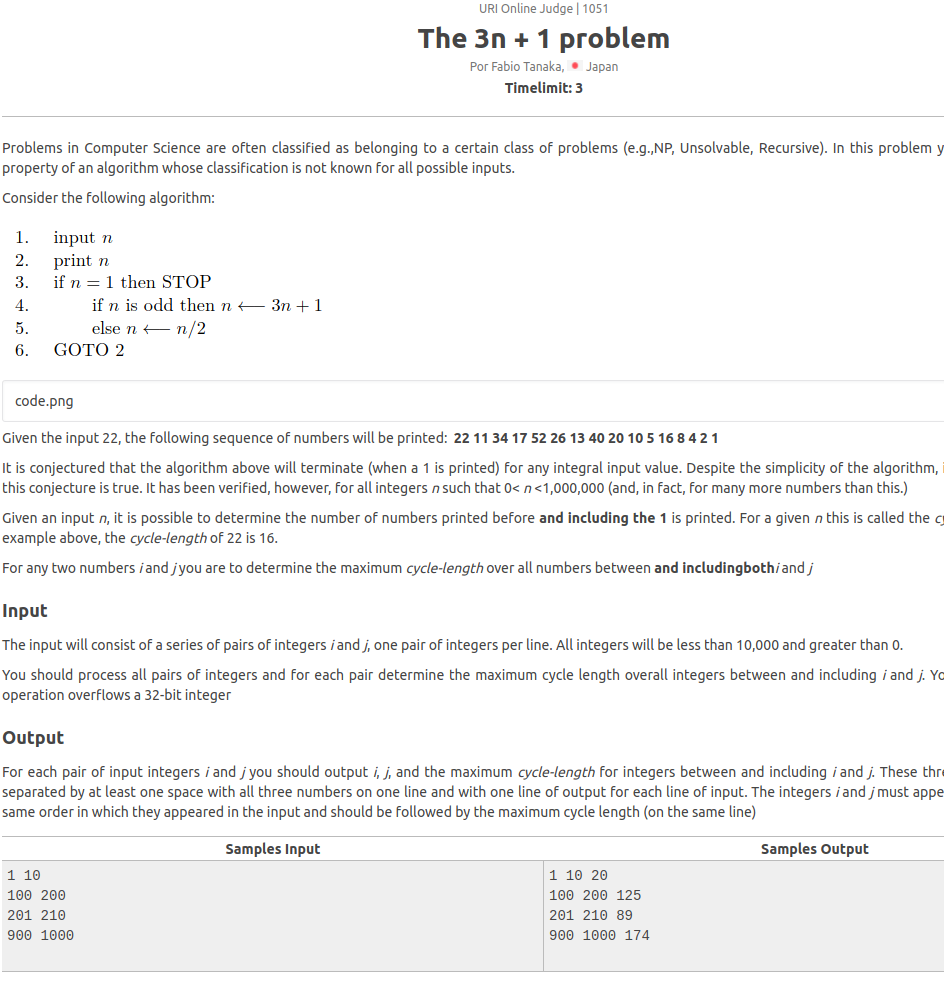
\includegraphics[width=1\textwidth]{img/3n_problem_label}
  \end{columns}
\end{frame}

\begin{frame}{Example: The 3n+1 problem}{What is the problem?}
  \begin{columns}
    \column{0.55\textwidth}
    {\smaller
    What is the longest sequence generated by this function?
      \begin{enumerate}
        \item input n
        \item if $n = 1$ then STOP
        \item if $n$ is odd, then $n = 3n + 1$
        \item else $n = n/2$
        \item GOTO 2
      \end{enumerate}

    For example, if $i = 1$ and $j = 4$:
    \begin{itemize}
      \item n = 1: 1 END; {\bf Length 1}
      \item n = 2: 2 1 END; {\bf Length 2}
      \item n = 3: 3 10 5 16 8 4 2 1 END; {\bf Length 8}
      \item n = 4: 4 2 1 END; {\bf Length 3}
    \end{itemize}
    So between n=1 and n=4, the maximum is 8 (n = 3)}
    \column{0.45\textwidth}
    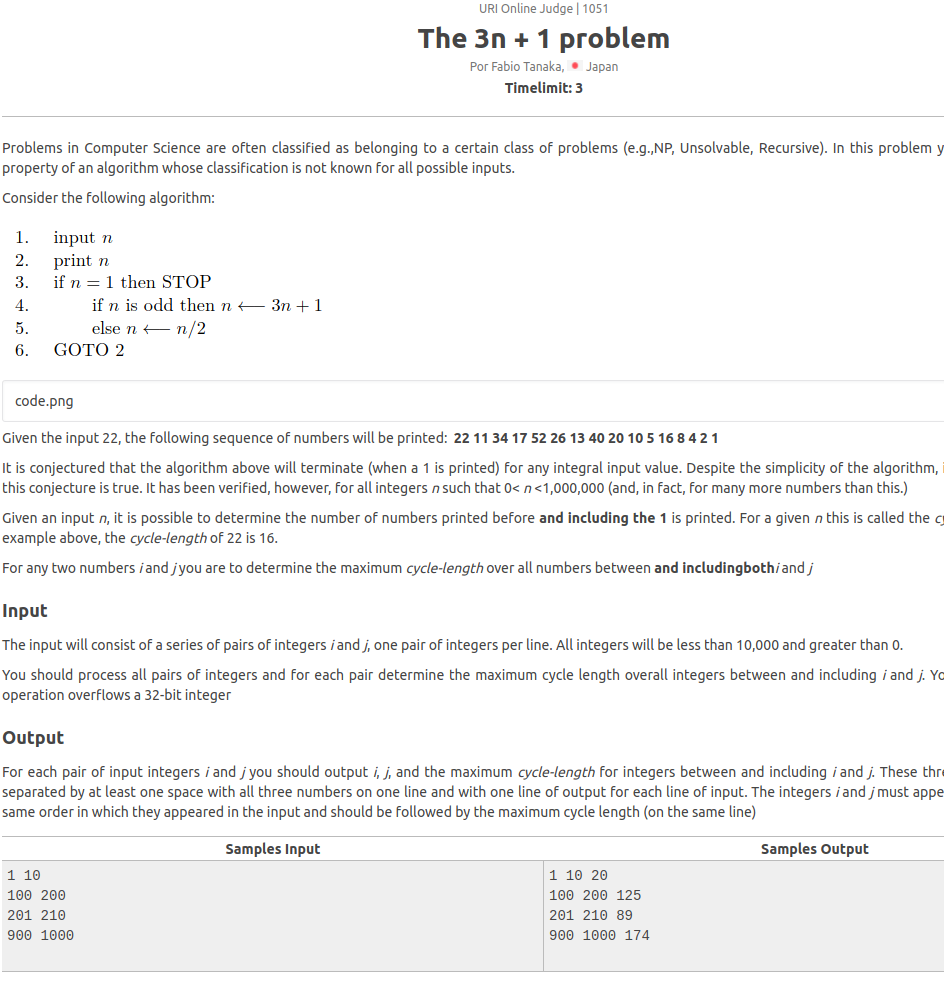
\includegraphics[width=1\textwidth]{img/3n_problem_label}
  \end{columns}
\end{frame}

\begin{frame}[fragile]{Example: The 3n+1 problem}{A simple program}
{\smaller
\begin{verbatim}
int main() {
  int min, max;
  int maxcycle = 0;
  cin >> min >> max;                           // Read i and j
  for (int a = min; a <= max; i++) {           // Loop from i to j
    int cycle = 1;               
    int n = a;
    while (n != 1) {
      if (n % 2 == 0) { n = n / 2; }           // calculate n
      else { n = n*3 + 1; }
      cycle++;                                 // increase cycle size
    }
    if (cycle > maxcycle) maxcycle = cycle;    // keep max cycle
  }
  cout << min << " " << max << " " << maxcycle << "\n";
  return 0;
}
\end{verbatim}}
\end{frame}

\begin{frame}{Example: The 3n+1 problem}{Simple programs, simple
  problems}

If you try to run this program with large inputs, it will be very slow! Why?
\bigskip

Consider the inputs: i = 1, j = 10:
\begin{itemize}
  \item n = 1: 1 END
  \item n = 2: 2 1 END
  ...
  \item n = 7: 7 22 11 34 17 52 26 13 40 20 10 5 16 8 4 2 1 END\\
  ...
  \item n = 9: 9 28 14 \alert{7 22 11 34 17 52 26 13 40 20 10 5 16 8 4 2 1 END}
  \item n = 10: \alert{10 5 16 8 4 2 1 END}
\end{itemize}
\bigskip

There is a lot of repetition!  How to make the program faster?
\end{frame}

\begin{frame}{Example: The 3n+1 problem}{Memoization}
  We use \alert{Memoization} to make the program faster
  \bigskip

  {\bf Memoization}:
  \begin{itemize}
    \item Every time you finish a calculation, store the result in the memory;
    \item Before you begin a calculation, check if the result is not in the memory;
  \end{itemize}
  \bigskip

  This technique can reduce the amount of repeated work.
  \bigskip

  In this course we will review and study many techniques like this one.\\
  You will have to implement these techniques in the homework to make it efficient.
\end{frame}

\subsection{Class Program}
\begin{frame}{Topics in this course}
  \begin{enumerate}
    \item Introduction
    \item Data Structures
    \item Search Problems
    \item Dynamic Programming
    \item Graphs Problems (Graph Structure)
    \item Graph Problems (Graph Search and Flow)
    \item String Manipulation
    \item Math Problems
    \item Geometry Problems
    \item Final Remix
  \end{enumerate}
\end{frame}

\subsection{Lecturer Introduction}
\begin{frame}
  \frametitle{About the Lecturer}
  \begin{columns}
    \column{0.4\textwidth}
    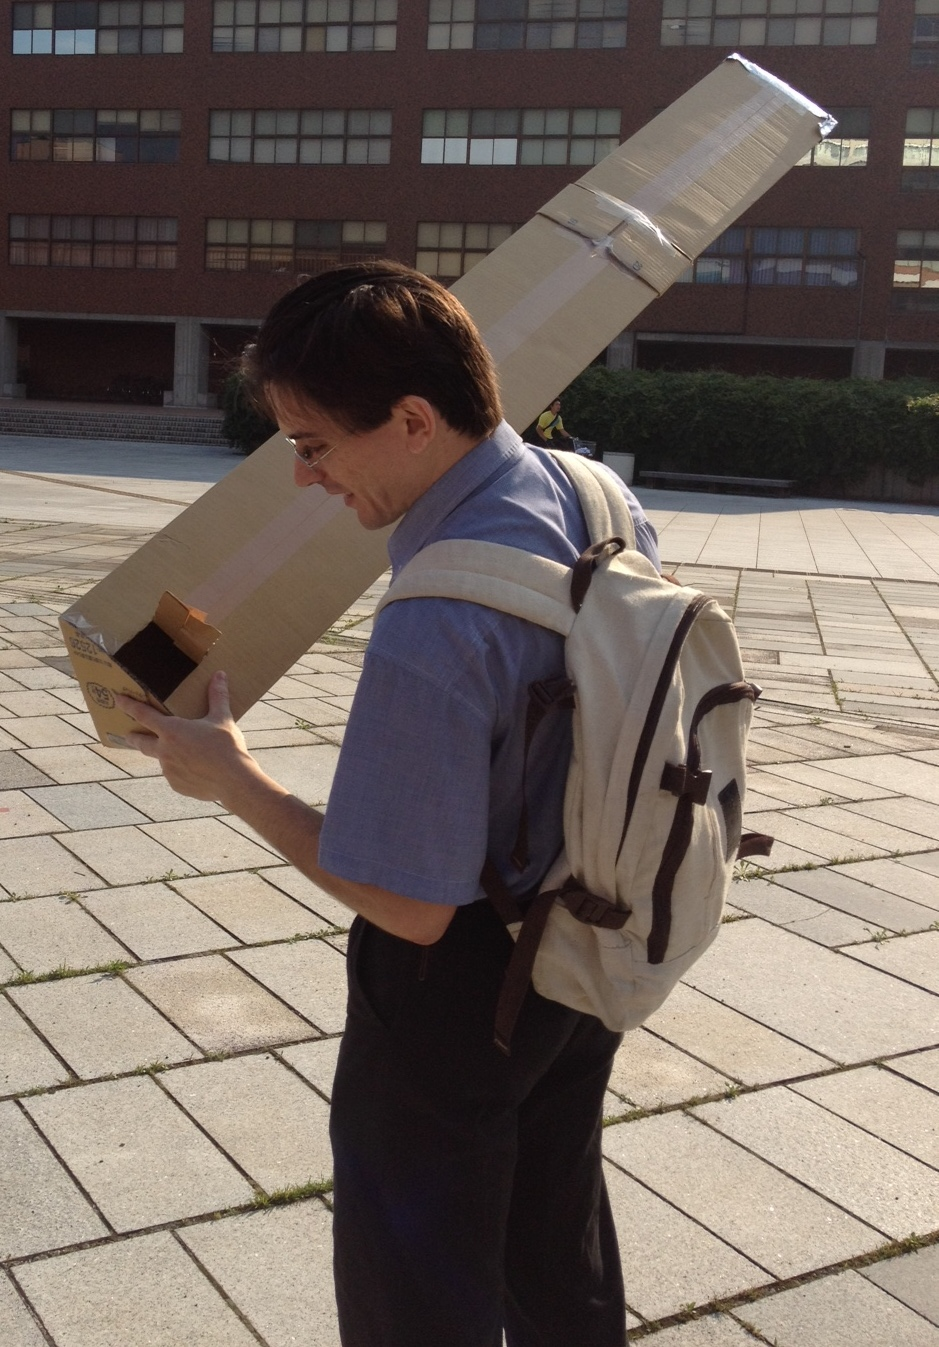
\includegraphics[height=.8\textheight]{../img/pinhole}
    \column{0.6\textwidth}
    {\small
    \begin{itemize}
      \item \structure{Name:} Claus Aranha;
      \item \structure{Country:} Brazil;
      \item \structure{Research Topics:}
      \begin{itemize}
        \item Evolutionary Computation;
        \item Artificial Life;
      \end{itemize}
      \item \structure{Hobbies:}
      \begin{itemize}
        \item Game Programming;
        \item Geocaching;
      \end{itemize}
        \medskip

      \item \structure{webpage:}\\ {\smaller \url{http://conclave.cs.tsukuba.ac.jp}}
    \end{itemize}
    }
  \end{columns}
\end{frame}

\begin{frame}{Why programming challenges?}
  \begin{itemize}
  \item {\bf For Competitions}: Competitive programming started around
    1980 in the US. Today, many universities in the world compete,
    including Tsukuba.
    \bigskip

  \item {\bf For Study}: Recently, many people use Automated Judges to
    study and improve programming ability (AtCoder, Codeforces, etc);
    \bigskip

  \item {\bf For Recruitment}: Also, many companies today use
    programming challenges in their recruitment.\bigskip

  \item {\bf For Fun}: It is fun to solve puzzles and to program!
  \end{itemize}
\end{frame}


\subsection{ICPC}
\begin{frame}{Extra: Join the Tsukuba ICPC Team!}{What is ICPC?}
  \hfill 
\includegraphics[width=0.4\textwidth]{img/icpclogo}\\
  If you like these contests, and want an extra challenge, please consider
  joining the Tsukuba ICPC team!
  \bigskip

  ICPC (International Collegiate Programming Contest) is the largest and
  most traditional programming competition between universities.
  \bigskip

  More than 50.000 students from all over the world participate in this
  competition every year.
  \bigskip

  Contest Website: \url{https://icpc.baylor.edu/}
\end{frame}

\begin{frame}{Extra: Join the Tsukuba ICPC Team!}{Program and see the world!}
  \hfill 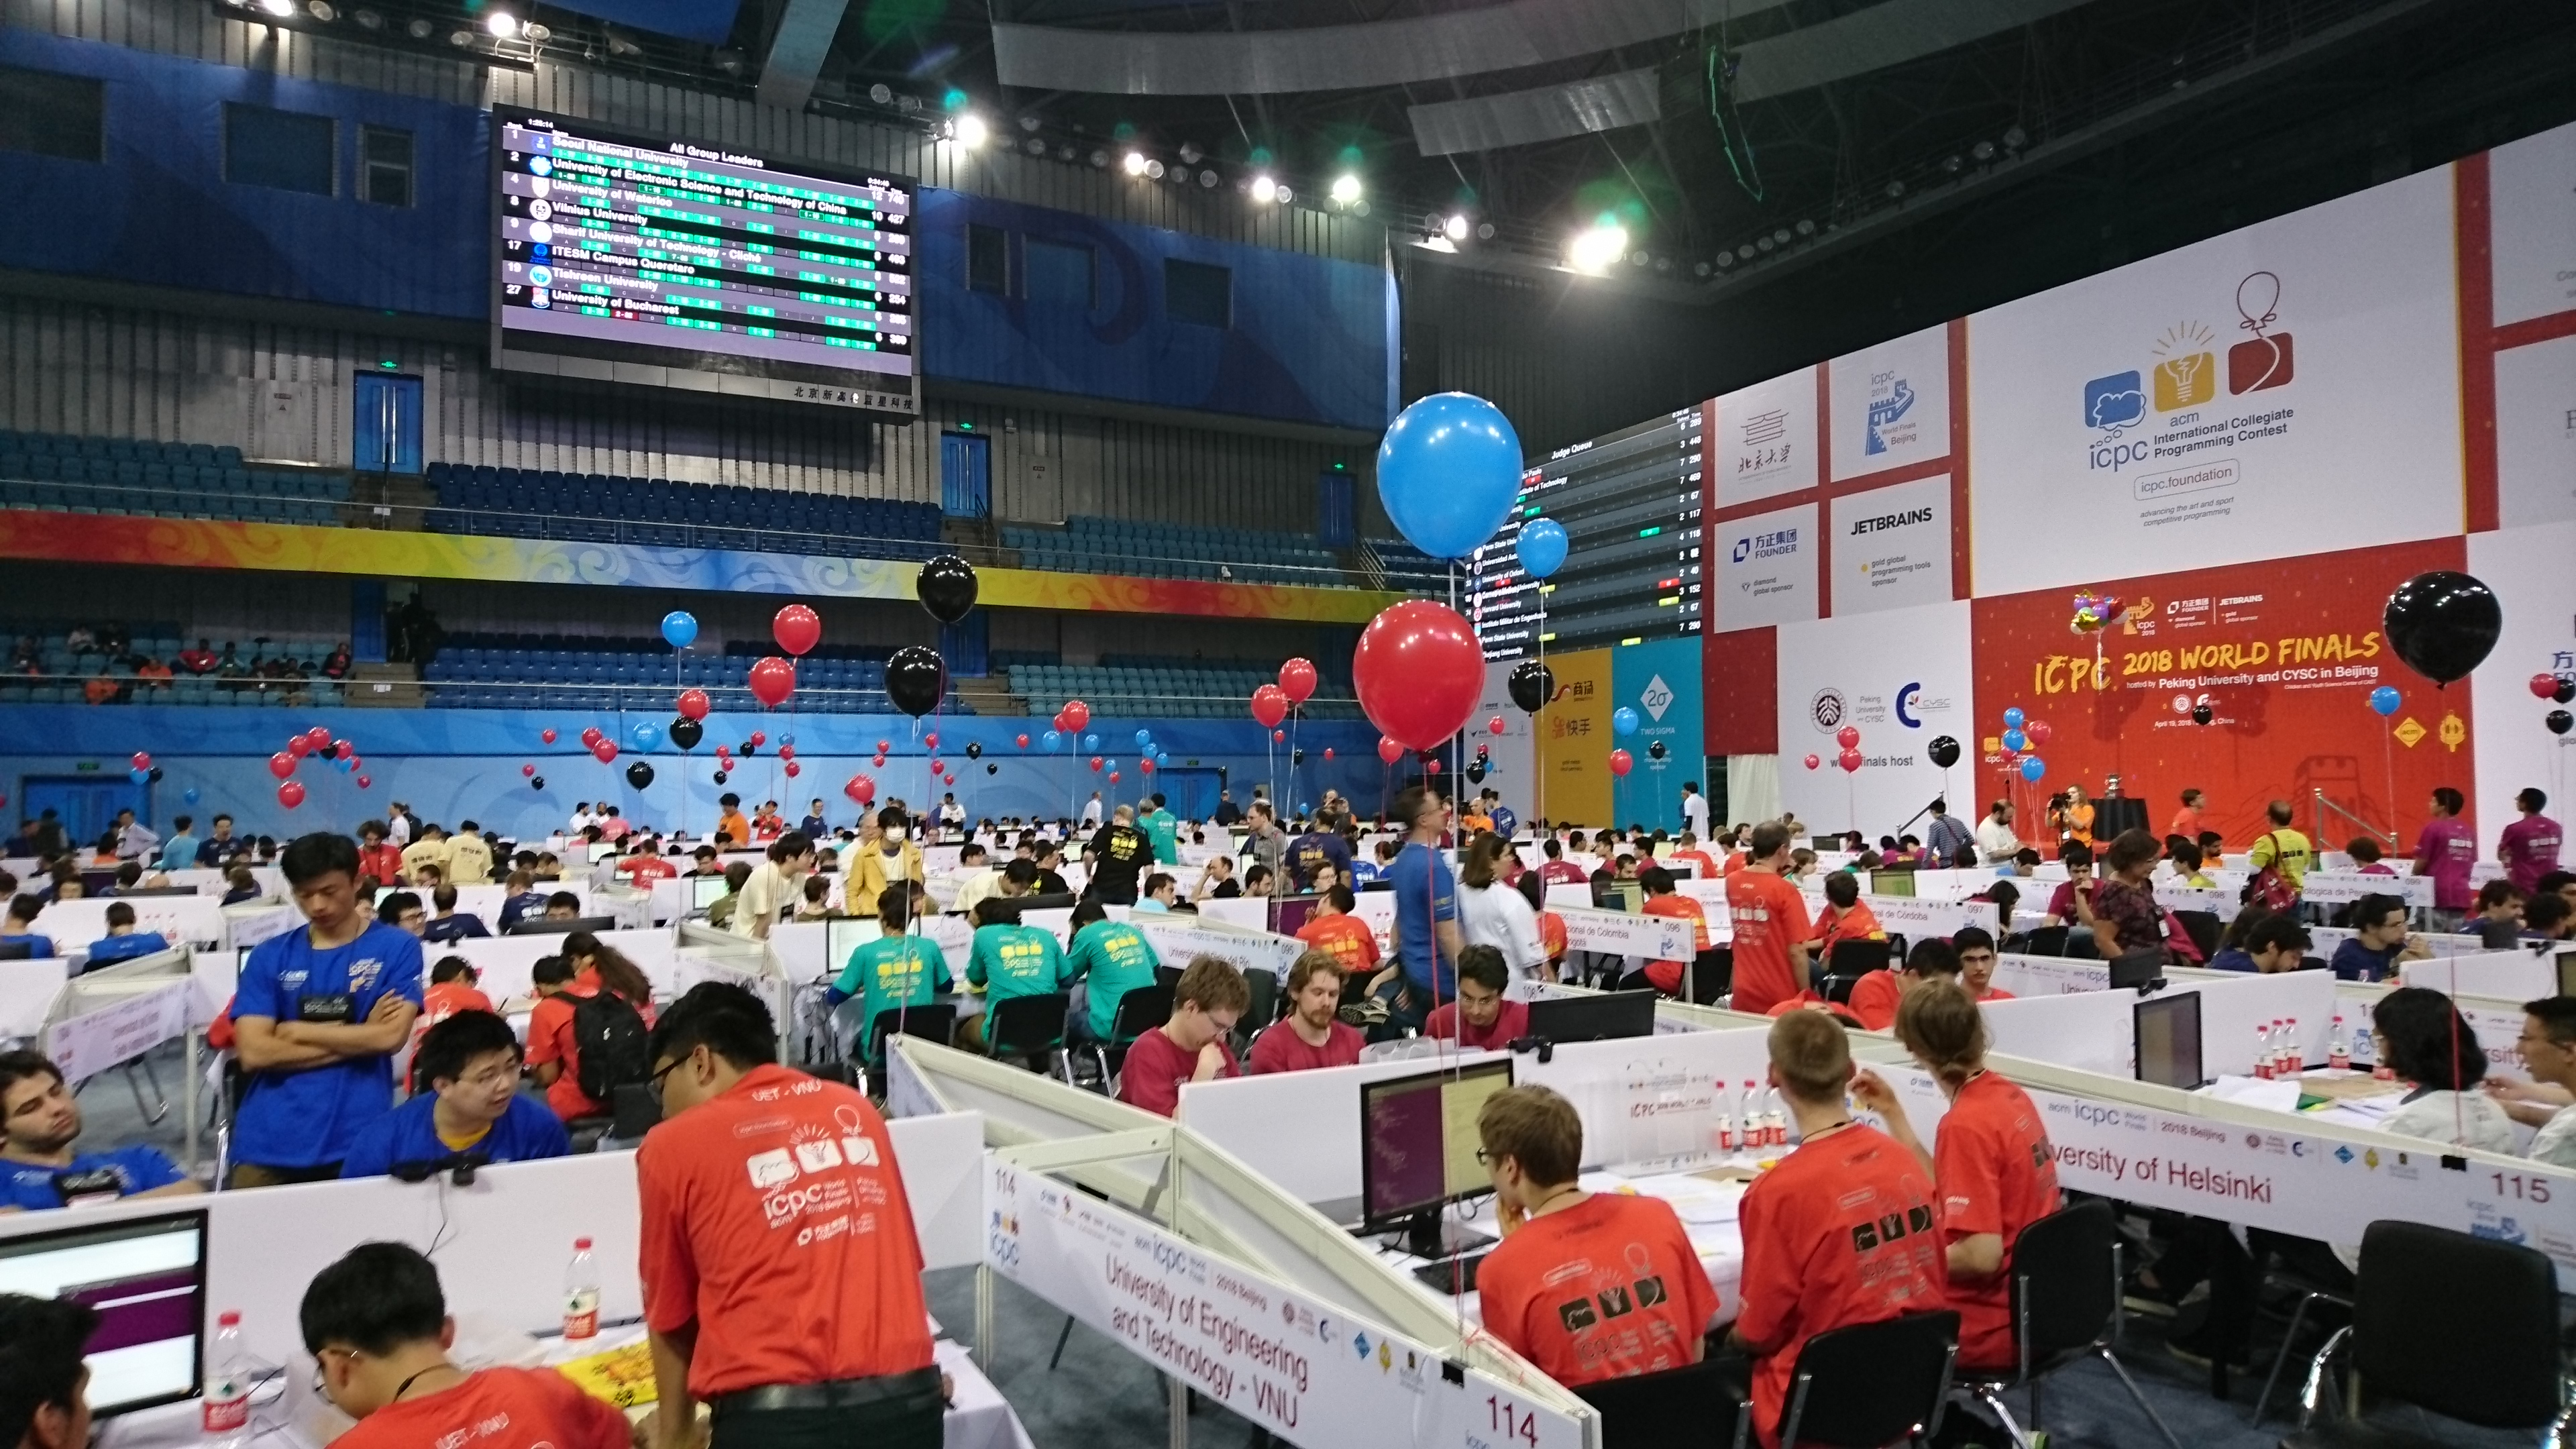
\includegraphics[width=0.4\textwidth]{img/icpc_image1}
  \begin{itemize}
    \item \alert{Requirements}: Team of 3 students, any course;
    \medskip

    \item \alert{Schedule:}
    \begin{itemize}
      \item First Online Contest in July
      \item Japanese National Contest in November
      \item World Final Next Year (June?)
    \end{itemize}
    \medskip
    \item Contact me if you're interested!
  \end{itemize}
\end{frame}



%%%%%%%%%%%%%%%%%%%%%%%%%%%%%%%%%%%%%%%%%%%%%%%%%%%%%%%%%%%%%%%%%%%%%%%%%%%%
